% Options for packages loaded elsewhere
% Options for packages loaded elsewhere
\PassOptionsToPackage{unicode}{hyperref}
\PassOptionsToPackage{hyphens}{url}
%
\documentclass[
  english,
  russian,
  12pt,
  a4paper,
  DIV=11,
  numbers=noendperiod]{scrreprt}
\usepackage{xcolor}
\usepackage{amsmath,amssymb}
\setcounter{secnumdepth}{5}
\usepackage{iftex}
\ifPDFTeX
  \usepackage[T1]{fontenc}
  \usepackage[utf8]{inputenc}
  \usepackage{textcomp} % provide euro and other symbols
\else % if luatex or xetex
  \usepackage{unicode-math} % this also loads fontspec
  \defaultfontfeatures{Scale=MatchLowercase}
  \defaultfontfeatures[\rmfamily]{Ligatures=TeX,Scale=1}
\fi
\usepackage{lmodern}
\ifPDFTeX\else
  % xetex/luatex font selection
\fi
% Use upquote if available, for straight quotes in verbatim environments
\IfFileExists{upquote.sty}{\usepackage{upquote}}{}
\IfFileExists{microtype.sty}{% use microtype if available
  \usepackage[]{microtype}
  \UseMicrotypeSet[protrusion]{basicmath} % disable protrusion for tt fonts
}{}
\usepackage{setspace}
% Make \paragraph and \subparagraph free-standing
\makeatletter
\ifx\paragraph\undefined\else
  \let\oldparagraph\paragraph
  \renewcommand{\paragraph}{
    \@ifstar
      \xxxParagraphStar
      \xxxParagraphNoStar
  }
  \newcommand{\xxxParagraphStar}[1]{\oldparagraph*{#1}\mbox{}}
  \newcommand{\xxxParagraphNoStar}[1]{\oldparagraph{#1}\mbox{}}
\fi
\ifx\subparagraph\undefined\else
  \let\oldsubparagraph\subparagraph
  \renewcommand{\subparagraph}{
    \@ifstar
      \xxxSubParagraphStar
      \xxxSubParagraphNoStar
  }
  \newcommand{\xxxSubParagraphStar}[1]{\oldsubparagraph*{#1}\mbox{}}
  \newcommand{\xxxSubParagraphNoStar}[1]{\oldsubparagraph{#1}\mbox{}}
\fi
\makeatother


\usepackage{longtable,booktabs,array}
\usepackage{calc} % for calculating minipage widths
% Correct order of tables after \paragraph or \subparagraph
\usepackage{etoolbox}
\makeatletter
\patchcmd\longtable{\par}{\if@noskipsec\mbox{}\fi\par}{}{}
\makeatother
% Allow footnotes in longtable head/foot
\IfFileExists{footnotehyper.sty}{\usepackage{footnotehyper}}{\usepackage{footnote}}
\makesavenoteenv{longtable}
\usepackage{graphicx}
\makeatletter
\newsavebox\pandoc@box
\newcommand*\pandocbounded[1]{% scales image to fit in text height/width
  \sbox\pandoc@box{#1}%
  \Gscale@div\@tempa{\textheight}{\dimexpr\ht\pandoc@box+\dp\pandoc@box\relax}%
  \Gscale@div\@tempb{\linewidth}{\wd\pandoc@box}%
  \ifdim\@tempb\p@<\@tempa\p@\let\@tempa\@tempb\fi% select the smaller of both
  \ifdim\@tempa\p@<\p@\scalebox{\@tempa}{\usebox\pandoc@box}%
  \else\usebox{\pandoc@box}%
  \fi%
}
% Set default figure placement to htbp
\def\fps@figure{htbp}
\makeatother



\ifLuaTeX
\usepackage[bidi=basic,provide=*]{babel}
\else
\usepackage[bidi=default,provide=*]{babel}
\fi
% get rid of language-specific shorthands (see #6817):
\let\LanguageShortHands\languageshorthands
\def\languageshorthands#1{}


\setlength{\emergencystretch}{3em} % prevent overfull lines

\providecommand{\tightlist}{%
  \setlength{\itemsep}{0pt}\setlength{\parskip}{0pt}}



 
\usepackage[style=gost-numeric,backend=biber,langhook=extras,autolang=other*]{biblatex}
\addbibresource{bib/cite.bib}

\usepackage[]{csquotes}

\usepackage{indentfirst}
\usepackage{float}
\floatplacement{figure}{H}
\IfFileExists{plex-otf.sty}{
  %% Full TeXlive
  \usepackage[
    % math,
    RM={Scale=0.94},SS={Scale=0.94},SScon={Scale=0.94},TT={Scale=MatchLowercase,FakeStretch=0.9},
    DefaultFeatures={Ligatures=Common}
  ]{plex-otf}
  \usepackage[Scale=MatchUppercase]{juliamono}
}{
  %% TinyTeX
  \usepackage{libertine}
}
\KOMAoption{captions}{tableheading}
\makeatletter
\@ifpackageloaded{caption}{}{\usepackage{caption}}
\AtBeginDocument{%
\ifdefined\contentsname
  \renewcommand*\contentsname{Содержание}
\else
  \newcommand\contentsname{Содержание}
\fi
\ifdefined\listfigurename
  \renewcommand*\listfigurename{Список иллюстраций}
\else
  \newcommand\listfigurename{Список иллюстраций}
\fi
\ifdefined\listtablename
  \renewcommand*\listtablename{Список таблиц}
\else
  \newcommand\listtablename{Список таблиц}
\fi
\ifdefined\figurename
  \renewcommand*\figurename{Рисунок}
\else
  \newcommand\figurename{Рисунок}
\fi
\ifdefined\tablename
  \renewcommand*\tablename{Таблица}
\else
  \newcommand\tablename{Таблица}
\fi
}
\@ifpackageloaded{float}{}{\usepackage{float}}
\floatstyle{ruled}
\@ifundefined{c@chapter}{\newfloat{codelisting}{h}{lop}}{\newfloat{codelisting}{h}{lop}[chapter]}
\floatname{codelisting}{Список}
\newcommand*\listoflistings{\listof{codelisting}{Листинги}}
\makeatother
\makeatletter
\makeatother
\makeatletter
\@ifpackageloaded{caption}{}{\usepackage{caption}}
\@ifpackageloaded{subcaption}{}{\usepackage{subcaption}}
\makeatother
	    \csundef{listoflistings}
	    
\makeatletter
\@ifpackageloaded{minted}{}{\usepackage[]{minted}}
\makeatother
	    \usemintedstyle{emacs}
	    \setminted{mathescape=true}
	    \setminted{autogobble=true}
	    \setminted{breaklines=true}
	    \setminted{breakanywhere=true}
	    \setminted{frame=lines}
	    % \setminted{bgcolor=lightgray}
	    %\setminted{linenos=true,
	    %  numberblanklines=false,
	    %}  
	    
\usepackage{bookmark}
\IfFileExists{xurl.sty}{\usepackage{xurl}}{} % add URL line breaks if available
\urlstyle{same}
\hypersetup{
  pdftitle={Шаблон отчёта по лабораторной работе №1},
  pdfauthor={Вакутайпа Милдред},
  pdflang={ru-RU},
  hidelinks,
  pdfcreator={LaTeX via pandoc}}


\title{Шаблон отчёта по лабораторной работе №1}
\usepackage{etoolbox}
\makeatletter
\providecommand{\subtitle}[1]{% add subtitle to \maketitle
  \apptocmd{\@title}{\par {\large #1 \par}}{}{}
}
\makeatother
\subtitle{Подготовка стенда}
\author{Вакутайпа Милдред}
\date{}
\begin{document}
\maketitle

\renewcommand*\contentsname{Содержание}
{
\setcounter{tocdepth}{1}
\tableofcontents
}
\listoffigures
\listoftables

\setstretch{1.5}
\chapter{Цель
работы}\label{ux446ux435ux43bux44c-ux440ux430ux431ux43eux442ux44b}

Цель данной работы - подготовить рабочее пространство и познакомиться с
языком программирования Julia и пакет DrWatson, освоить основы
литературного программирования.

\chapter{Задание}\label{ux437ux430ux434ux430ux43dux438ux435}

\begin{enumerate}
\def\labelenumi{\arabic{enumi}.}
\item
  Создать рабочий каталог для всего курса.
\item
  Создать рабочее пространство для программ в рамках лабораторной
  работы.
\item
  Выполнить все задания по тексту лабораторной работы.
\item
  Установить необходимые пакеты.
\item
  Выполнить предложенный код.
\item
  Преобразовать код в литературный стиль.
\item
  Сгенерировать из литературного кода:

  --- чистый код;

  --- jupyter notebook;

  --- документацию в формате Quarto.
\item
  Выполнить код из jupyter notebook.
\item
  Интегрировать документацию в формате Quarto в отчёт.
\item
  Добавить в код в литературном стиле вычисление для набора параметров.
\item
  Сгенерировать из литературного кода с параметрами:

  --- чистый код;

  --- jupyter notebook;

  --- документацию в формате Quarto.

  --- Выполнить код из jupyter notebook с параметрами.

  --- Интегрировать документацию с параметрами в формате Quarto в отчёт.
\end{enumerate}

\chapter{Выполнение лабораторной
работы}\label{ux432ux44bux43fux43eux43bux43dux435ux43dux438ux435-ux43bux430ux431ux43eux440ux430ux442ux43eux440ux43dux43eux439-ux440ux430ux431ux43eux442ux44b}

\section{Настройка
git}\label{ux43dux430ux441ux442ux440ux43eux439ux43aux430-git}

Сначла установила git, чтобы работать с системой контроля версии github
локально и gh ,чтобы работать в командной строке.

\begin{figure}

\centering{

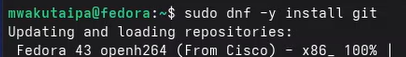
\includegraphics[width=0.7\linewidth,height=\textheight,keepaspectratio]{image/1.png}

}

\caption{\label{fig-001}Установка git}

\end{figure}%

\begin{figure}

\centering{

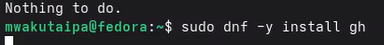
\includegraphics[width=0.7\linewidth,height=\textheight,keepaspectratio]{image/2.png}

}

\caption{\label{fig-002}Установка gh}

\end{figure}%

Далее я вошла в свою учетную запись в командной строке зададив свой
логин и email.

\begin{figure}

\centering{

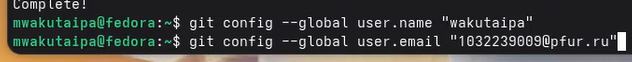
\includegraphics[width=0.7\linewidth,height=\textheight,keepaspectratio]{image/3.png}

}

\caption{\label{fig-003}Настройки git}

\end{figure}%

Настроила utf-8 в выводе сообщений git, верификацию и подписание
комммитов. Задддала имя начальной ветки (master) и настроила autocrlf и
safecrlf.

\begin{figure}

\centering{

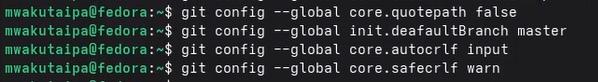
\includegraphics[width=0.7\linewidth,height=\textheight,keepaspectratio]{image/4.png}

}

\caption{\label{fig-004}Настройки git}

\end{figure}%

Потом я создала аккаунт на gitverse и вошла в существующий аккаунт
github

\begin{figure}

\centering{

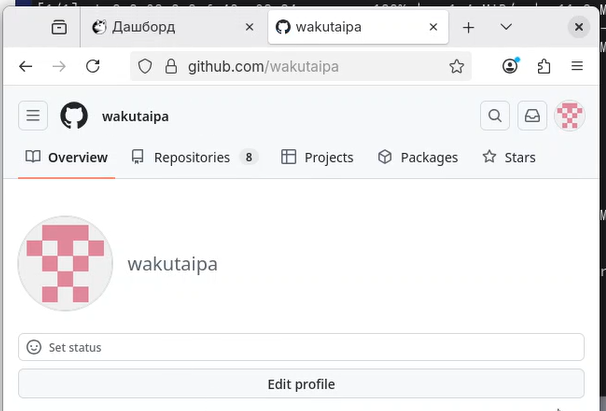
\includegraphics[width=0.7\linewidth,height=\textheight,keepaspectratio]{image/5.png}

}

\caption{\label{fig-005}Профиль github}

\end{figure}%

\begin{figure}

\centering{

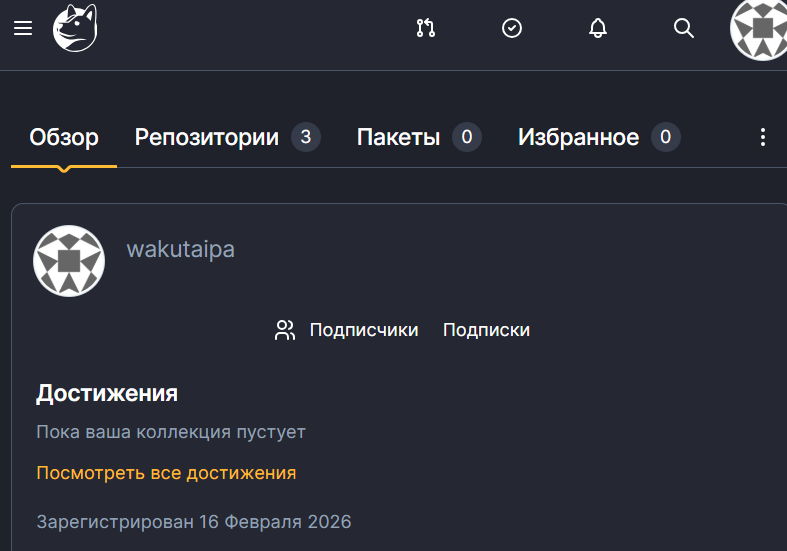
\includegraphics[width=0.7\linewidth,height=\textheight,keepaspectratio]{image/8.png}

}

\caption{\label{fig-008}Профиль gitverse}

\end{figure}%

Авторизировалась с gh через броузер

\begin{figure}

\centering{

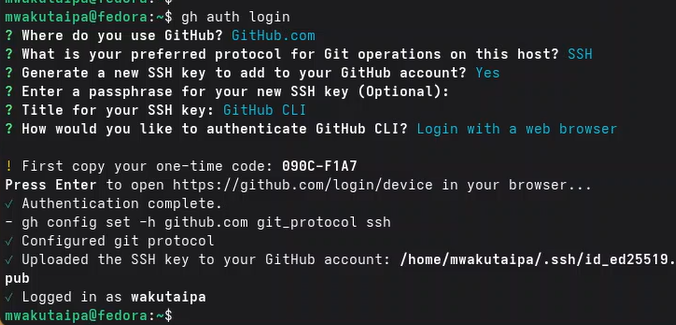
\includegraphics[width=0.7\linewidth,height=\textheight,keepaspectratio]{image/6.png}

}

\caption{\label{fig-006}Авторизаться gh}

\end{figure}%

\begin{figure}

\centering{

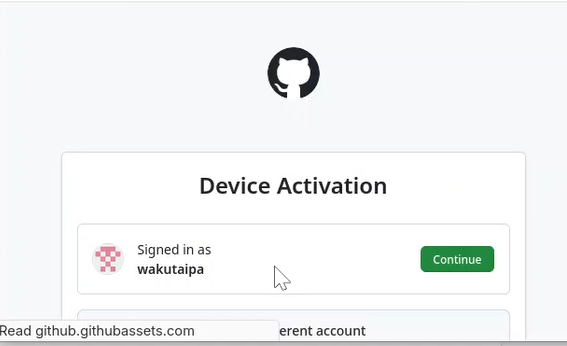
\includegraphics[width=0.7\linewidth,height=\textheight,keepaspectratio]{image/7.png}

}

\caption{\label{fig-007}Авторизаться в броузере}

\end{figure}%

Создала ssh ключ для доступа к github и добавила в агент. Добавила ключ
в учетную запись gitverse через web-интерфейс после коприрования с
помощью xclip.

\begin{figure}

\centering{

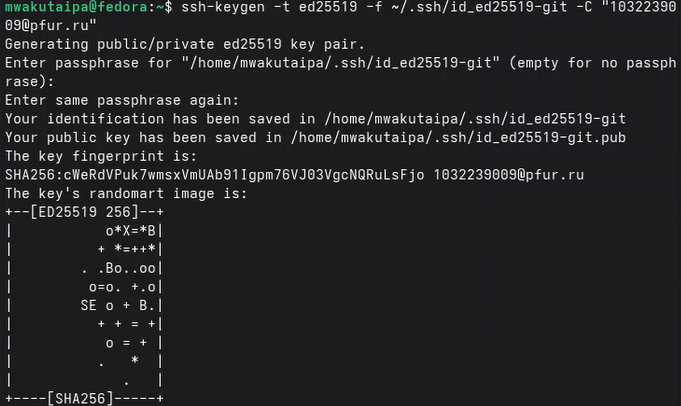
\includegraphics[width=0.7\linewidth,height=\textheight,keepaspectratio]{image/9.png}

}

\caption{\label{fig-009}Создание ключ ssh}

\end{figure}%

\begin{figure}

\centering{

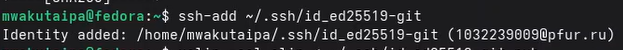
\includegraphics[width=0.7\linewidth,height=\textheight,keepaspectratio]{image/10.png}

}

\caption{\label{fig-010}Добавление ключ к учетную запись github}

\end{figure}%

\begin{figure}

\centering{

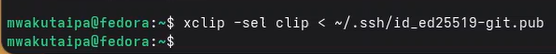
\includegraphics[width=0.7\linewidth,height=\textheight,keepaspectratio]{image/11.png}

}

\caption{\label{fig-011}Копирование ключа}

\end{figure}%

\begin{figure}

\centering{


\includegraphics[width=0.7\linewidth,height=\textheight,keepaspectratio]{image/12.png}

}

\caption{\label{fig-012}Добавление ключ к gitverse}

\end{figure}%

Сгенерировала ключ gpg типа RSA and RSA, размера 4096, срока действия по
умолчанию (не истекает никогда). Задала имя и электронную почту
соответствущему адресу и на github и на gitverse

\begin{figure}

\centering{

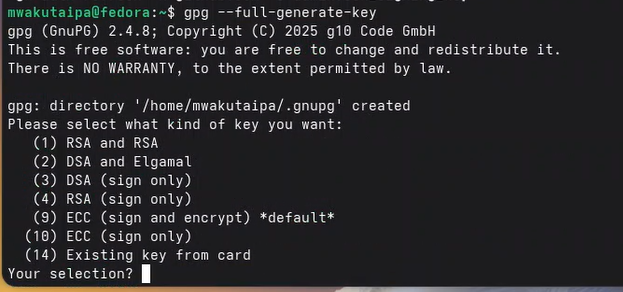
\includegraphics[width=0.7\linewidth,height=\textheight,keepaspectratio]{image/13.png}

}

\caption{\label{fig-013}Создание ключа gpg}

\end{figure}%

Выводила список ключей и скопировала отпечаток приватного ключа в буфер
обмена и вставила полученный ключ и на github и на giverse.

\begin{figure}

\centering{

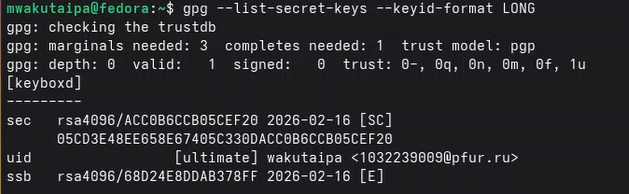
\includegraphics[width=0.7\linewidth,height=\textheight,keepaspectratio]{image/14.png}

}

\caption{\label{fig-014}Список ключей}

\end{figure}%

\begin{figure}

\centering{


\includegraphics[width=0.7\linewidth,height=\textheight,keepaspectratio]{image/15.png}

}

\caption{\label{fig-015}Копирование опечаток}

\end{figure}%

\begin{figure}

\centering{

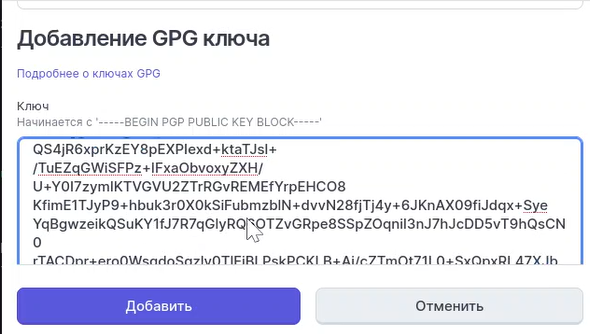
\includegraphics[width=0.7\linewidth,height=\textheight,keepaspectratio]{image/16.png}

}

\caption{\label{fig-016}Добавление ключа на gitverse}

\end{figure}%

\begin{figure}

\centering{

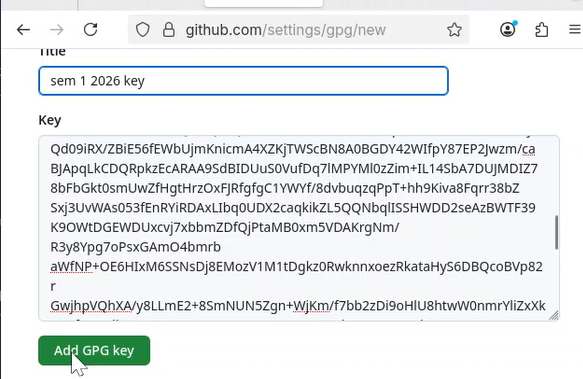
\includegraphics[width=0.7\linewidth,height=\textheight,keepaspectratio]{image/17.png}

}

\caption{\label{fig-017}Добавление ключа на github}

\end{figure}%

Используя введёный email, указала Git применять его при подписи
коммитов.

\begin{figure}

\centering{

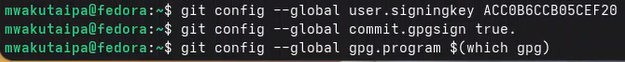
\includegraphics[width=0.7\linewidth,height=\textheight,keepaspectratio]{image/18.png}

}

\caption{\label{fig-018}Настройка автоматических подписей коммитов git}

\end{figure}%

\section{Рабочее пространство лабораторной
работы}\label{ux440ux430ux431ux43eux447ux435ux435-ux43fux440ux43eux441ux442ux440ux430ux43dux441ux442ux432ux43e-ux43bux430ux431ux43eux440ux430ux442ux43eux440ux43dux43eux439-ux440ux430ux431ux43eux442ux44b}

Установила средства разработки

\begin{figure}

\centering{

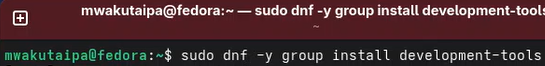
\includegraphics[width=0.7\linewidth,height=\textheight,keepaspectratio]{image/19.png}

}

\caption{\label{fig-019}Установка dev-tools}

\end{figure}%

Из COPR установила quarto

\begin{figure}

\centering{

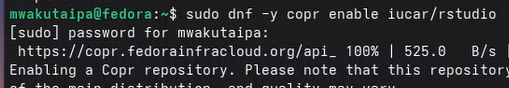
\includegraphics[width=0.7\linewidth,height=\textheight,keepaspectratio]{image/20.png}

}

\caption{\label{fig-020}Установка quarto}

\end{figure}%

\begin{figure}

\centering{

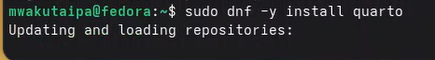
\includegraphics[width=0.7\linewidth,height=\textheight,keepaspectratio]{image/21.png}

}

\caption{\label{fig-021}Установка quarto}

\end{figure}%

\begin{figure}

\centering{

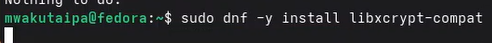
\includegraphics[width=0.7\linewidth,height=\textheight,keepaspectratio]{image/22.png}

}

\caption{\label{fig-022}Установка quarto}

\end{figure}%

На Node.js базируется программное обеспечение для семантического вер-
сионирования и общепринятых коммитов, позтому установила nodejs и для
управления пакетами установила pnpm и yarn

\begin{figure}

\centering{

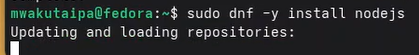
\includegraphics[width=0.7\linewidth,height=\textheight,keepaspectratio]{image/23.png}

}

\caption{\label{fig-023}Установка Nodejs}

\end{figure}%

\begin{figure}

\centering{

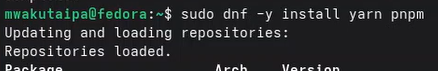
\includegraphics[width=0.7\linewidth,height=\textheight,keepaspectratio]{image/24.png}

}

\caption{\label{fig-024}Установка pnpm и yarn}

\end{figure}%

Для работы с Node.js добавила каталог с исполняемыми файлами,
устанавлива- емыми пакетным менеджером, в переменную PATH.

\begin{figure}

\centering{

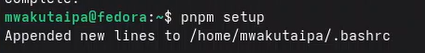
\includegraphics[width=0.7\linewidth,height=\textheight,keepaspectratio]{image/25.png}

}

\caption{\label{fig-025}pnpm setup}

\end{figure}%

\begin{figure}

\centering{

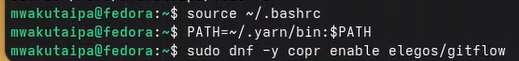
\includegraphics[width=0.7\linewidth,height=\textheight,keepaspectratio]{image/26.png}

}

\caption{\label{fig-026}Запуск pnpm}

\end{figure}%

В файле \textasciitilde/.bashrc добавила к переменной PATH yarn и
установила gitflow из COPR

\begin{figure}

\centering{

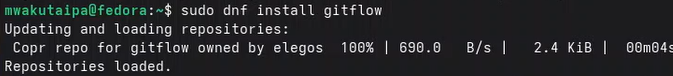
\includegraphics[width=0.7\linewidth,height=\textheight,keepaspectratio]{image/27.png}

}

\caption{\label{fig-027}Установка gitflow}

\end{figure}%

Commitizen используется для помощи в форматировании коммитов. Установила
его и с pnpm и с yarn

\begin{figure}

\centering{

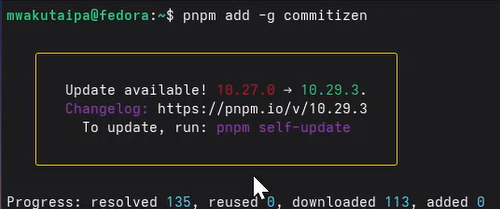
\includegraphics[width=0.7\linewidth,height=\textheight,keepaspectratio]{image/28.png}

}

\caption{\label{fig-028}Установка commitizen с pnpm}

\end{figure}%

\begin{figure}

\centering{

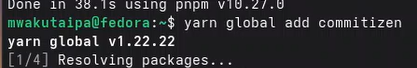
\includegraphics[width=0.7\linewidth,height=\textheight,keepaspectratio]{image/29.png}

}

\caption{\label{fig-029}Установка commitizen с yarn}

\end{figure}%

cz-customizable позволяет более глубоко настроить форматирование
коммитов. Устанавила его с pnpm

\begin{figure}

\centering{

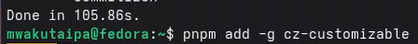
\includegraphics[width=0.7\linewidth,height=\textheight,keepaspectratio]{image/30.png}

}

\caption{\label{fig-030}Установка cz-customizable с pnpm}

\end{figure}%

standard-version автоматизирует изменение номера версии. Нстановила его
с pnpm и yarn

\begin{figure}

\centering{

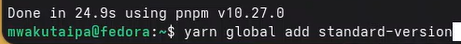
\includegraphics[width=0.7\linewidth,height=\textheight,keepaspectratio]{image/31.png}

}

\caption{\label{fig-031}Установка standard-version}

\end{figure}%

Создала репозиторий на основе шаблона в gitverse и сделала его
публичным.

\begin{figure}

\centering{

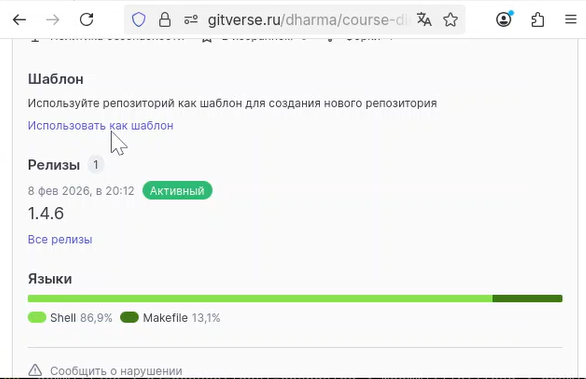
\includegraphics[width=0.7\linewidth,height=\textheight,keepaspectratio]{image/33.png}

}

\caption{\label{fig-032}Создание репозиторий из шаблона}

\end{figure}%

\begin{figure}

\centering{

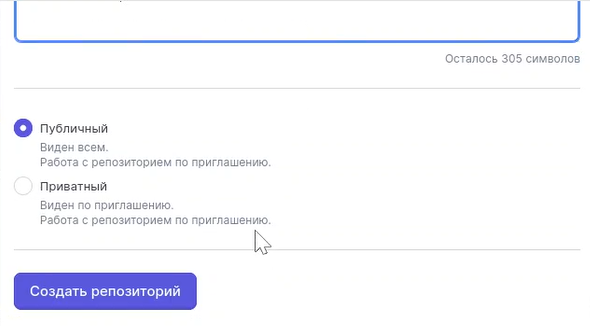
\includegraphics[width=0.7\linewidth,height=\textheight,keepaspectratio]{image/34.png}

}

\caption{\label{fig-033}Настройки репозиторий}

\end{figure}%

Потом я создала директорию для моей работы, клонировала репозиторий и
инициализировала курс.

\begin{figure}

\centering{

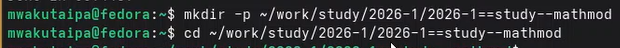
\includegraphics[width=0.7\linewidth,height=\textheight,keepaspectratio]{image/36.png}

}

\caption{\label{fig-034}Создание директории}

\end{figure}%

\begin{figure}

\centering{

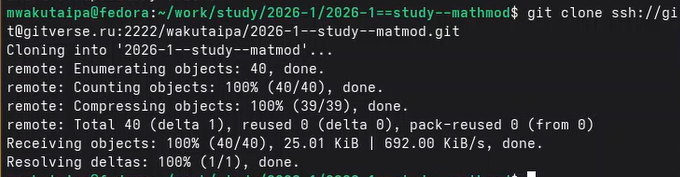
\includegraphics[width=0.7\linewidth,height=\textheight,keepaspectratio]{image/38.png}

}

\caption{\label{fig-035}Клонирование в директорию}

\end{figure}%

Потом я отправила файлы на сервер.

\begin{figure}

\centering{

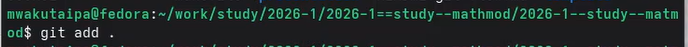
\includegraphics[width=0.7\linewidth,height=\textheight,keepaspectratio]{image/40.png}

}

\caption{\label{fig-037}git add}

\end{figure}%

\begin{figure}

\centering{

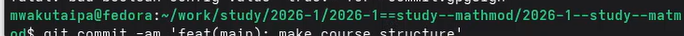
\includegraphics[width=0.7\linewidth,height=\textheight,keepaspectratio]{image/41.png}

}

\caption{\label{fig-038}git commit}

\end{figure}%

\begin{figure}

\centering{

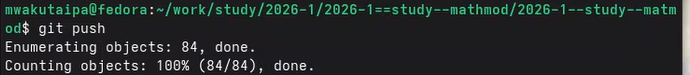
\includegraphics[width=0.7\linewidth,height=\textheight,keepaspectratio]{image/42.png}

}

\caption{\label{fig-039}git push}

\end{figure}%

Я создала новый репозиторий в github и запускала репозиторий на github.

\begin{figure}

\centering{

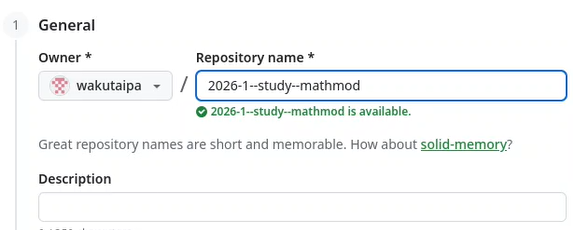
\includegraphics[width=0.7\linewidth,height=\textheight,keepaspectratio]{image/39.png}

}

\caption{\label{fig-036}Создание репозиторий в github}

\end{figure}%

\begin{figure}

\centering{

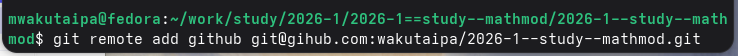
\includegraphics[width=0.7\linewidth,height=\textheight,keepaspectratio]{image/44.png}

}

\caption{\label{fig-040}Добавление пользователя github}

\end{figure}%

\begin{figure}

\centering{

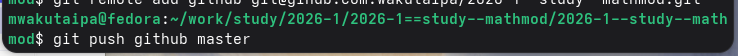
\includegraphics[width=0.7\linewidth,height=\textheight,keepaspectratio]{image/45.png}

}

\caption{\label{fig-041}Отправка файлы на сервер}

\end{figure}%

Инициализировала git-flow, который мне понадобиться для работы.

\begin{figure}

\centering{

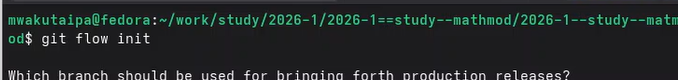
\includegraphics[width=0.7\linewidth,height=\textheight,keepaspectratio]{image/43.png}

}

\caption{\label{fig-042}Инициализирование git-flow}

\end{figure}%

Проверила на какой ветке нахожусь

\begin{figure}

\centering{

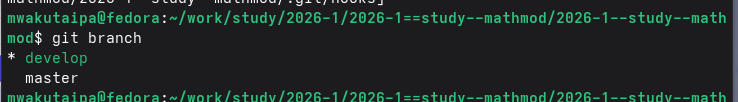
\includegraphics[width=0.7\linewidth,height=\textheight,keepaspectratio]{image/46.png}

}

\caption{\label{fig-043}Ветки}

\end{figure}%

Загрузила весь репозиторий в хранилище

\begin{figure}

\centering{

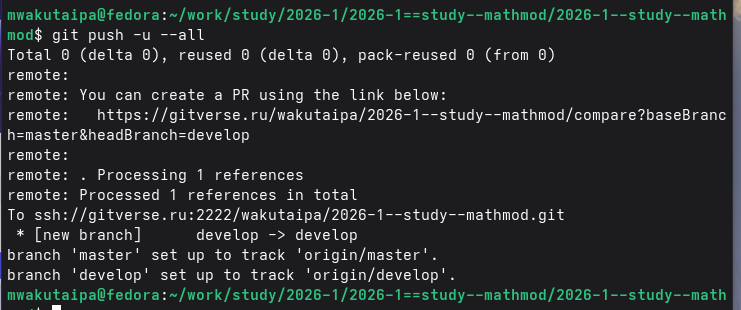
\includegraphics[width=0.7\linewidth,height=\textheight,keepaspectratio]{image/47.png}

}

\caption{\label{fig-044}Загрузка репозиторий в хранилище}

\end{figure}%

Создала перый релиз (версия 1.0.0) и перешла на ветку release

\begin{figure}

\centering{

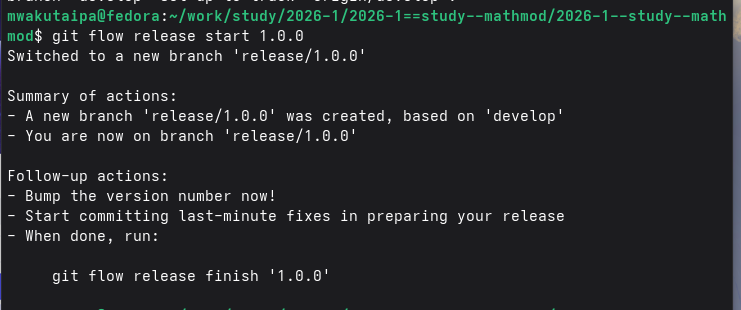
\includegraphics[width=0.7\linewidth,height=\textheight,keepaspectratio]{image/48.png}

}

\caption{\label{fig-045}Релиз 1.0.0}

\end{figure}%

Создадала журнал изменений

\begin{figure}

\centering{

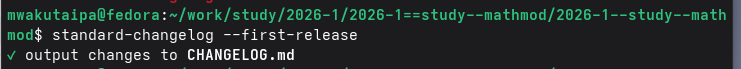
\includegraphics[width=0.7\linewidth,height=\textheight,keepaspectratio]{image/50.png}

}

\caption{\label{fig-046}Создание журнала изменений}

\end{figure}%

Добавила журнал изменений в индекс и сохранила сообщение мерджа как и
было

\begin{figure}

\centering{

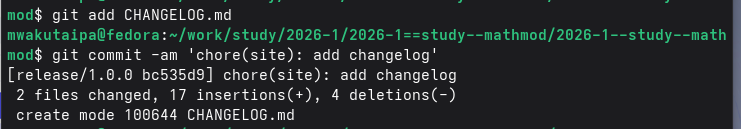
\includegraphics[width=0.7\linewidth,height=\textheight,keepaspectratio]{image/51.png}

}

\caption{\label{fig-047}Добавление журнала изменений}

\end{figure}%

\begin{figure}

\centering{

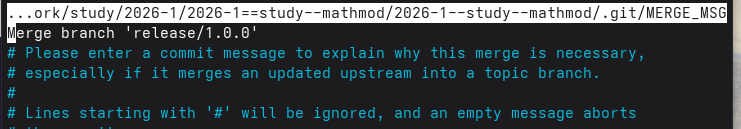
\includegraphics[width=0.7\linewidth,height=\textheight,keepaspectratio]{image/52.png}

}

\caption{\label{fig-048}Merge msg}

\end{figure}%

Залила релизную ветку в основную ветку

\begin{figure}

\centering{

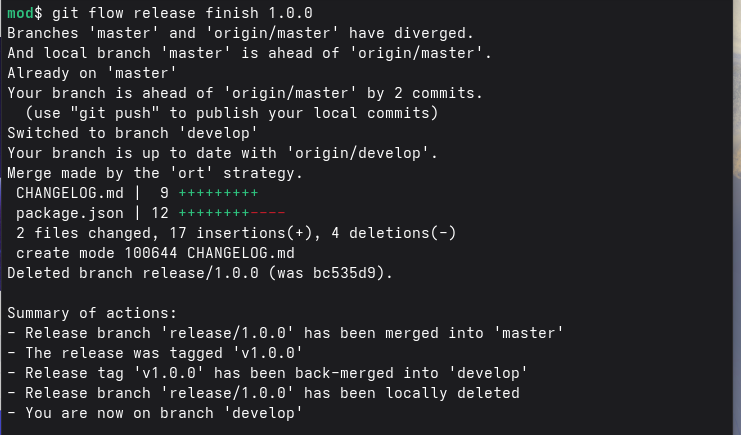
\includegraphics[width=0.7\linewidth,height=\textheight,keepaspectratio]{image/53.png}

}

\caption{\label{fig-048}Добаление ветку в основную}

\end{figure}%

Отправила данные на github

\begin{figure}

\centering{

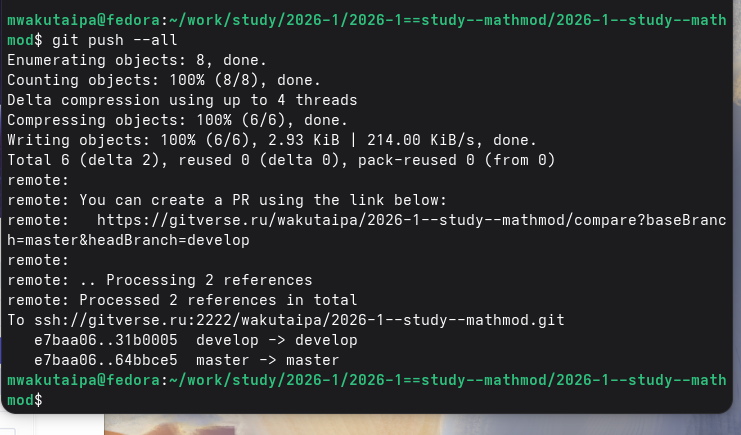
\includegraphics[width=0.7\linewidth,height=\textheight,keepaspectratio]{image/54.png}

}

\caption{\label{fig-049}Отправка данных на github}

\end{figure}%

\begin{figure}

\centering{

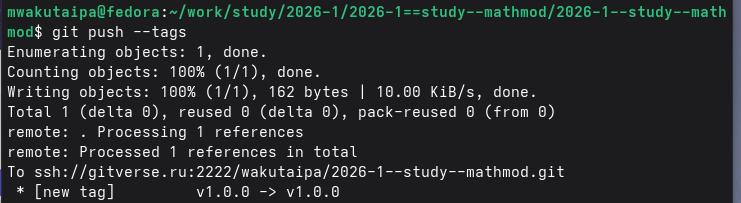
\includegraphics[width=0.7\linewidth,height=\textheight,keepaspectratio]{image/55.png}

}

\caption{\label{fig-050}Отправка данных на github}

\end{figure}%

Скопировала CHANGELOG.md в каталог release

\begin{figure}

\centering{

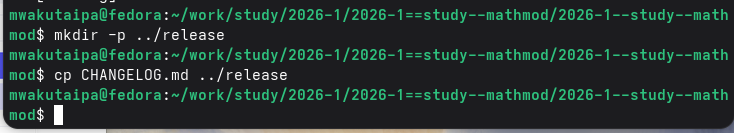
\includegraphics[width=0.7\linewidth,height=\textheight,keepaspectratio]{image/56.png}

}

\caption{\label{fig-051}копирование в каталог release}

\end{figure}%

Создала релиз с использованием утилиты работы с github

\begin{figure}

\centering{

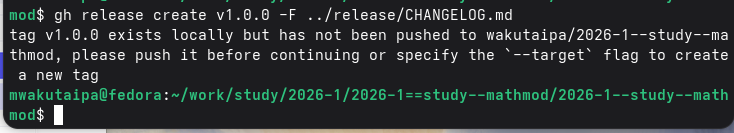
\includegraphics[width=0.7\linewidth,height=\textheight,keepaspectratio]{image/57.png}

}

\caption{\label{fig-052}Создание релиза}

\end{figure}%

\section{Создание проекта DrWatson для лабораторных
работ}\label{ux441ux43eux437ux434ux430ux43dux438ux435-ux43fux440ux43eux435ux43aux442ux430-drwatson-ux434ux43bux44f-ux43bux430ux431ux43eux440ux430ux442ux43eux440ux43dux44bux445-ux440ux430ux431ux43eux442}

Перешла в каталог labs/lab01 и в терминале запускала Julia

\begin{figure}

\centering{

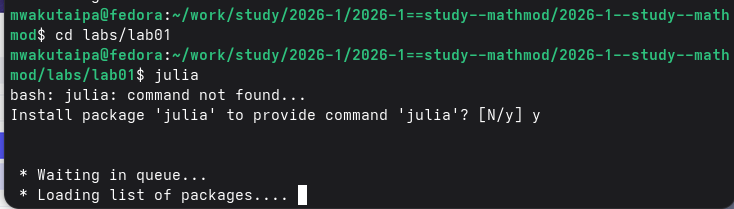
\includegraphics[width=0.7\linewidth,height=\textheight,keepaspectratio]{image/58.png}

}

\caption{\label{fig-053}каталог lab01}

\end{figure}%

В REPL иннициализировала проект DrWatson

\begin{figure}

\centering{

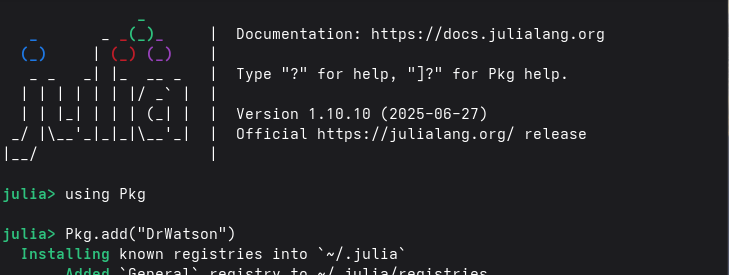
\includegraphics[width=0.7\linewidth,height=\textheight,keepaspectratio]{image/60.png}

}

\caption{\label{fig-054}иннициализирование DrWatson}

\end{figure}%

\begin{figure}

\centering{

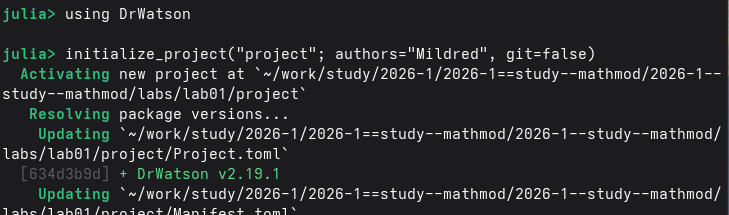
\includegraphics[width=0.7\linewidth,height=\textheight,keepaspectratio]{image/61.png}

}

\caption{\label{fig-055}иннициализирование DrWatson}

\end{figure}%

Перешла в созданный каталог и позтапно установила основные пакеты

\begin{figure}

\centering{

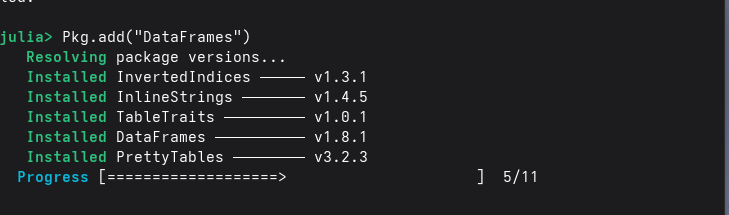
\includegraphics[width=0.7\linewidth,height=\textheight,keepaspectratio]{image/62.png}

}

\caption{\label{fig-055}Установка DataFrames}

\end{figure}%

\begin{figure}

\centering{

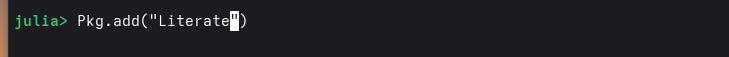
\includegraphics[width=0.7\linewidth,height=\textheight,keepaspectratio]{image/63.png}

}

\caption{\label{fig-056}Установка Literate}

\end{figure}%

\begin{figure}

\centering{

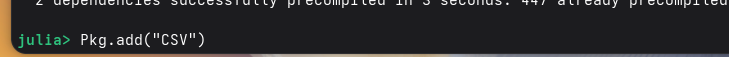
\includegraphics[width=0.7\linewidth,height=\textheight,keepaspectratio]{image/64.png}

}

\caption{\label{fig-057}Установка CSV}

\end{figure}%

\begin{figure}

\centering{

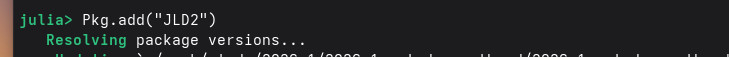
\includegraphics[width=0.7\linewidth,height=\textheight,keepaspectratio]{image/65.png}

}

\caption{\label{fig-058}Установка JLD2}

\end{figure}%

\begin{figure}

\centering{

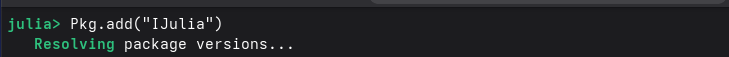
\includegraphics[width=0.7\linewidth,height=\textheight,keepaspectratio]{image/66.png}

}

\caption{\label{fig-059}Установка IJulia}

\end{figure}%

\begin{figure}

\centering{

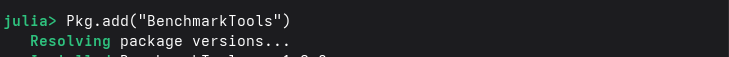
\includegraphics[width=0.7\linewidth,height=\textheight,keepaspectratio]{image/67.png}

}

\caption{\label{fig-060}Установка BenchmarkTools}

\end{figure}%

\begin{figure}

\centering{


\includegraphics[width=0.7\linewidth,height=\textheight,keepaspectratio]{image/68.png}

}

\caption{\label{fig-061}Установка Quarto}

\end{figure}%

Создала тестовый скрипт scripts/test\_setup.jl, чтобы проверить
установки

\begin{figure}

\centering{

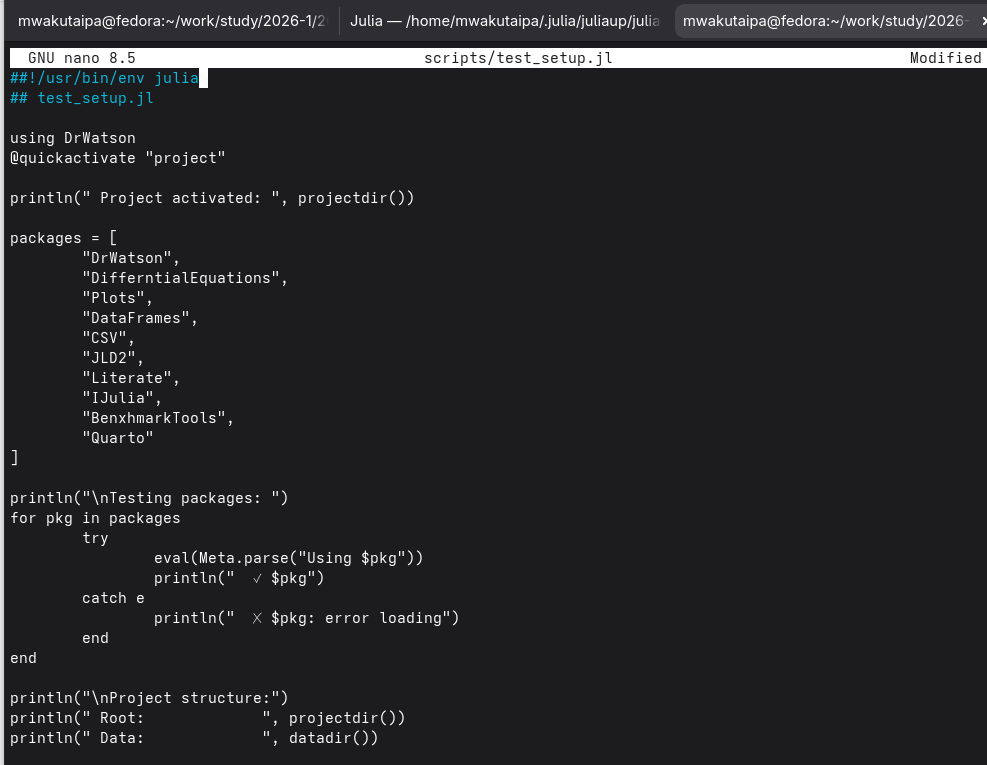
\includegraphics[width=0.7\linewidth,height=\textheight,keepaspectratio]{image/69.png}

}

\caption{\label{fig-062}скрит для тетирования}

\end{figure}%

\begin{minted}{julia}

##!/usr/bin/env julia
## test_setup.jl

using DrWatson
@quickactivate "project"
println("✅ Проект активирован: ", projectdir())
## Проверка пакетов
packages = [
    "DrWatson", # Организация проекта
    "DifferentialEquations", # Решение ОДУ
    "Plots",    # Визуализация
    "DataFrames",   # Таблицы данных
    "CSV",  # Работа с CSV
    "JLD2", # Сохранение данных
    "Literate", # Literate programming
    "IJulia",   # Jupyter notebook
    "BenchmarkTools",   # Бенчмаркинг
    "Quarto"    # Создание отчетов
    ]
println("\nПроверка пакетов:")
for pkg in packages
    try
        eval(Meta.parse("using $pkg"))
        println(" ✓ $pkg")
    catch e
        println(" ✗ $pkg: Ошибка загрузки")
    end
end
## Проверка путей
println("\nСтруктура проекта:")
println(" Корень:   ", projectdir())
println(" Данные:   ", datadir())
println(" Скрипты:  ", srcdir())
println(" Графики:  ", plotsdir())


\end{minted}

Потом запускала скрипт

\begin{figure}

\centering{

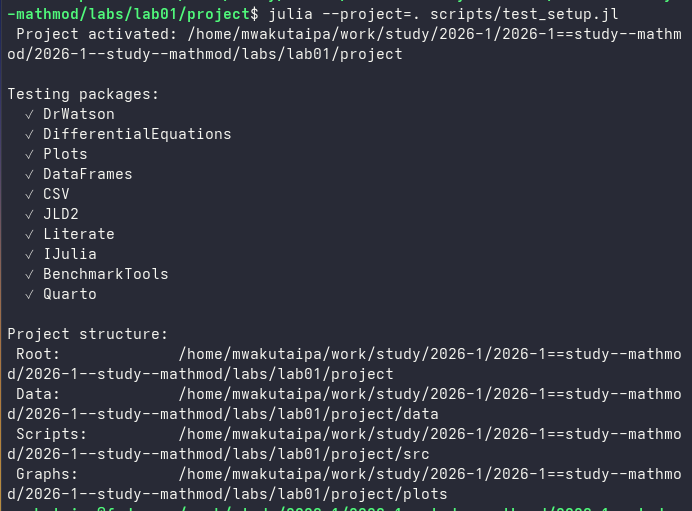
\includegraphics[width=0.7\linewidth,height=\textheight,keepaspectratio]{image/72.png}

}

\caption{\label{fig-063}Прверка установки со скриптом}

\end{figure}%

\section{Модель экспоненциального
роста}\label{ux43cux43eux434ux435ux43bux44c-ux44dux43aux441ux43fux43eux43dux435ux43dux446ux438ux430ux43bux44cux43dux43eux433ux43e-ux440ux43eux441ux442ux430}

Экспоненциальный рост --- это процесс увеличения величины, при котором
ско- рость роста в каждый момент времени пропорциональна текущему
значению этой величины. Чем больше система, тем быстрее она растет.
Создала скрипт (scripts/01\_exponential\_growth.jl) и запускала его.

\begin{minted}{julia}

using DrWatson
@quickactivate "project"

using DifferentialEquations
using Plots
using DataFrames

function exponential_growth!(du, u, p, t)
    α = p
    du[1] = α * u[1]
end
u0 = [1.0]  # начальная популяция
α = 0.3 # скорость роста
tspan = (0.0, 10.0) # временной интервал

prob = ODEProblem(exponential_growth!, u0, tspan, α)
sol = solve(prob, Tsit5(), saveat=0.1)

plot(sol, label="u(t)", xlabel="Время t", ylabel="Популяция u",
    title="Экспоненциальный рост (α = $α)", lw=2, legend=:topleft)
    
savefig(plotsdir("exponential_growth_α=$α.png"))

df = DataFrame(t=sol.t, u=first.(sol.u))
println("Первые 5 строк результатов:")
println(first(df, 5))

u_final = last(sol.u)[1]
doubling_time = log(2) / α
println("\nАналитическое время удвоения: ", round(doubling_time; digits=2))

\end{minted}

\begin{figure}

\centering{

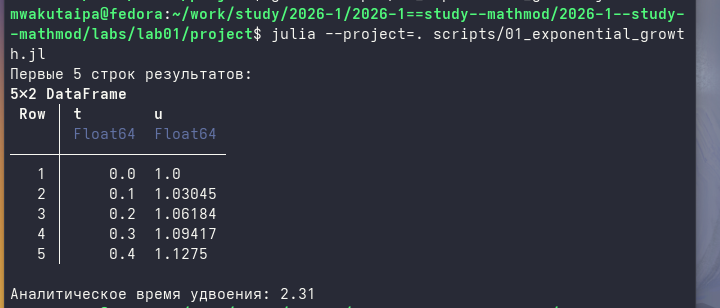
\includegraphics[width=0.7\linewidth,height=\textheight,keepaspectratio]{image/75.png}

}

\caption{\label{fig-064}Запуск скрипта 01\_exponential\_growth.jl}

\end{figure}%

\begin{figure}

\centering{

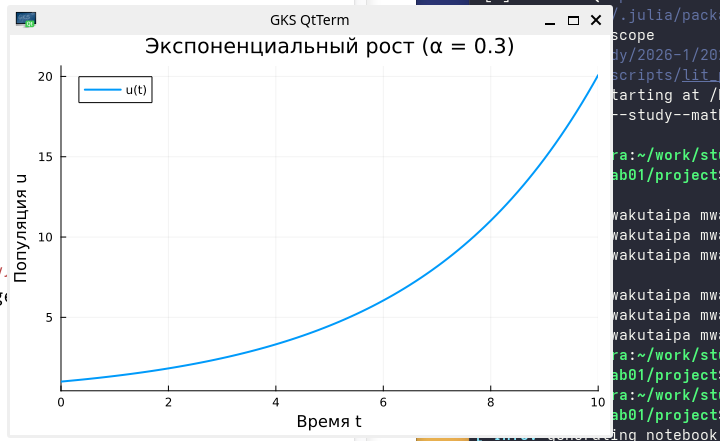
\includegraphics[width=0.7\linewidth,height=\textheight,keepaspectratio]{image/76.png}

}

\caption{\label{fig-065}Созданный график}

\end{figure}%

Изменила файл scripts/01\_exponential\_growth.lj:

\begin{minted}{julia}

# # Экспоненциальный рост
# **Цель:** Исследовать решение уравнения 𝑑𝑢/𝑑𝑡 = 𝛼𝑢.
#
# ## Инициализация проекта и загрузка пакетов

using DrWatson
@quickactivate "project"

using DifferentialEquations
using Plots
using DataFrames
using JLD2

script_name = splitext(basename(PROGRAM_FILE))[1]
mkpath(plotsdir(script_name))
mkpath(datadir(script_name))
# ## Определение модели
# Уравнение экспоненциального роста:
# 𝑑𝑢/𝑑𝑡 = 𝛼𝑢, 𝑢(0) = 𝑢0

function exponential_growth!(du, u, p, t)
    α = p
    du[1] = α * u[1]
end

u0 = [1.0]  # начальная популяция
α = 0.3     # скорость роста
tspan = (0.0, 10.0) # временной интервал

prob = ODEProblem(exponential_growth!, u0, tspan, α)
sol = solve(prob, Tsit5(), saveat=0.1)

plot(sol, label="u(t)", xlabel="Время t", ylabel="Популяция u",
    title="Экспоненциальный рост (α = $α)", lw=2, legend=:topleft)

savefig(plotsdir("exponential_growth_α=$α.png"))

df = DataFrame(t=sol.t, u=first.(sol.u))
println("Первые 5 строк результатов:")
println(first(df, 5))

u_final = last(sol.u)[1]
doubling_time = log(2) / α
println("\nАналитическое время удвоения: ", round(doubling_time; digits=2))

@save datadir(script_name, "all_results.jld2") df


\end{minted}

Выполнила программный код:

\begin{figure}

\centering{

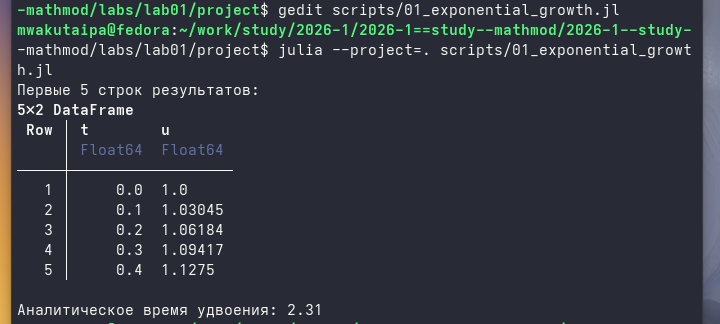
\includegraphics[width=0.7\linewidth,height=\textheight,keepaspectratio]{image/79.png}

}

\caption{\label{fig-066}Выполнение кода}

\end{figure}%

Создала скрипт для генерации производных форматов (scripts/tangle.jl):

\begin{minted}{julia}

#!/usr/bin/env julia
# tangle.jl - Генератор отчетов из Literate-скриптов
# Использование: julia tangle.jl <путь_к_скрипту>
using DrWatson
@quickactivate

# Активирует текущий проект DrWatson
using Literate

function main()
        if length(ARGS) == 0
            println("""
                Использование: julia tangle.jl <путь_к_скрипту>
                Примеры:
                julia tangle.jl scripts/lab1.jl
                """)
            return
        end

    script_path = ARGS[1]

    if !isfile(script_path)
        error("Файл не найден: $script_path")
    end

# Пути и имена
    script_dir = dirname(script_path)
    script_name = splitext(basename(script_path))[1]

    println("Генерация из: $script_path")

# Чистый скрипт (без комментариев)
    scripts_dir = scriptsdir(script_name)
    Literate.script(script_path, scripts_dir; credit=false)
    println(" ✓ Чистый скрипт: $(scripts_dir)/$(script_name).jl")

# Quarto-документ
    quarto_dir = projectdir("markdown", script_name);
    Literate.markdown(script_path, quarto_dir;
            flavor=Literate.QuartoFlavor(),
            name=script_name, credit=false)
    println("✓ Quarto: $(quarto_dir)/$(script_name).qmd")

# Jupyter notebook
    notebooks_dir = projectdir("notebooks", script_name)
    Literate.notebook(script_path, notebooks_dir, name=script_name;
                execute=false, credit=false)
    println(" ✓ Notebook: $(notebooks_dir)/$(script_name).ipynb")
    println("\nГотово! Все файлы созданы.")
end

# Запуск
if abspath(PROGRAM_FILE) == @__FILE__
    main()
end

\end{minted}

Потом выполнила программу, чтобы создать производные форматы

\begin{figure}

\centering{

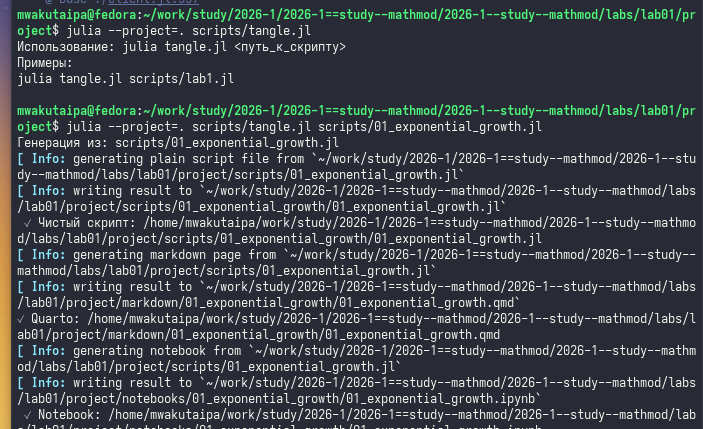
\includegraphics[width=0.7\linewidth,height=\textheight,keepaspectratio]{image/81.png}

}

\caption{\label{fig-067}Выполнение tangle.jl}

\end{figure}%

В каталоге отчёта в файл \_quarto.yml включила поддержку кода julia.

\begin{figure}

\centering{

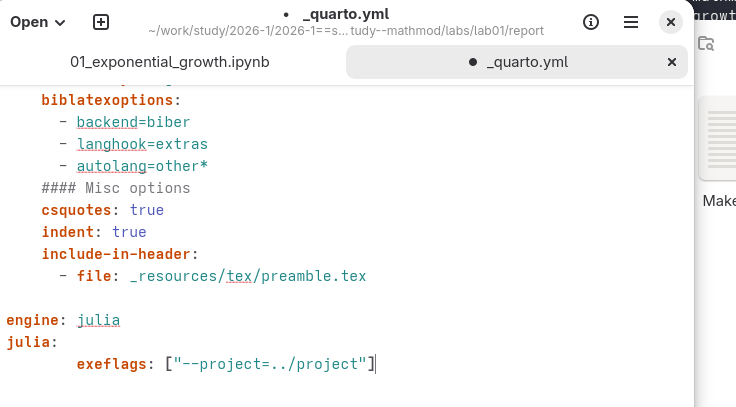
\includegraphics[width=0.7\linewidth,height=\textheight,keepaspectratio]{image/83.png}

}

\caption{\label{fig-068}Включение поддержку julia}

\end{figure}%

В преамбуле preamble.tex подключила пакет juliamono

\begin{figure}

\centering{

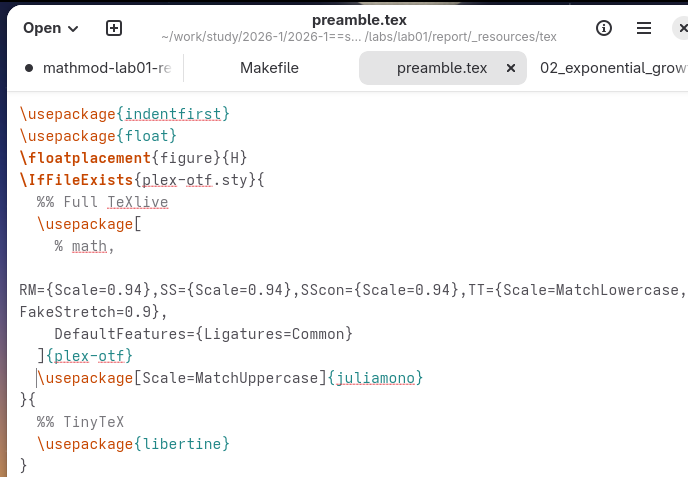
\includegraphics[width=0.7\linewidth,height=\textheight,keepaspectratio]{image/ы.png}

}

\caption{\label{fig-069}Включение пакет juliamono}

\end{figure}%

Исследование не ограничивается одним значением параметров, поэтому
изменила программу так, чтобы она принимала набор параметров.

\begin{minted}{julia}

# # Параметрическое исследование экспоненциального роста
#
# ## Активация проекта и загрузка пакетов
#
# **ИЗМЕНЕНИЕ:** Добавлен DrWatson для управления проектом и параметрами

using DrWatson
@quickactivate "project"    # Активация проекта DrWatson

using DifferentialEquations
using DataFrames
using Plots
using JLD2
using BenchmarkTools

# Установка каталогов
script_name = splitext(basename(PROGRAM_FILE))[1]
mkpath(plotsdir(script_name))
mkpath(datadir(script_name))

# ## Определение модели
# Модель: 𝑑𝑢/𝑑𝑡 = 𝛼 ⋅ 𝑢

function exponential_growth!(du, u, p, t)
    α = p.α # **ИЗМЕНЕНИЕ:** Параметры теперь передаются как именованный кортеж
    du[1] = α * u[1]
end

# ## Определение параметров в Dict
# **ОСНОВНОЕ ИЗМЕНЕНИЕ:** Все параметры собраны в Dict для систематизации
# Базовый набор параметров (один эксперимент)

base_params = Dict(
    :u0 => [1.0],   # начальная популяция
    :α => 0.3,  # скорость роста
    :tspan => (0.0, 10.0), # интервал времени
    :solver => Tsit5(), # метод решения
    :saveat => 0.1, # шаг сохранения результатов
    :experiment_name => "base_experiment"
    )
    
println("Базовые параметры эксперимента:")
for (key, value) in base_params
    println(" $key = $value")
end

# ## Функция-обертка для запуска одного эксперимента
# **ИСПРАВЛЕНИЕ:** Возвращаем Dict со строковыми ключами

function run_single_experiment(params::Dict)
    @unpack u0, α, tspan, solver, saveat = params
    prob = ODEProblem(exponential_growth!, u0, tspan, (α=α,)) #Создаем и решаем задачу
    sol = solve(prob, solver; saveat=saveat)
    final_population = last(sol.u)[1] # Анализ результатов
    doubling_time = log(2) / α
    return Dict(
        "solution" => sol,
        "time_points" => sol.t,
        "population_values" => first.(sol.u),
        "final_population" => final_population,
        "doubling_time" => doubling_time,
        "parameters" => params # Сохраняем исходные параметры
        ) # Используем строки как ключи для совместимости с DrWatson
end

# ## Запуск базового эксперимента
# **ИЗМЕНЕНИЕ:** Используем produce_or_load для автоматического кэширования

data, path = produce_or_load(
        datadir(script_name, "single"), # Папка для сохранения
        base_params,    # Параметры эксперимента
        run_single_experiment, # Функция для выполнения
        prefix = "exp_growth", # Префикс имени файла
        tag = false, # Не добавлять git-тег
        verbose = true
        )
        
println("\nРезультаты базового эксперимента:")
println(" Финальная популяция: ", data["final_population"])
println(" Время удвоения: ", round(data["doubling_time"]; digits=2))

# ## Визуализация базового эксперимента
p1 = plot(data["time_points"], data["population_values"],
        label="α = $(base_params[:α])",
        xlabel="Время, t",
        ylabel="Популяция, u(t)",
        title="Экспоненциальный рост (базовый эксперимент)",
        lw=2,
        legend=:topleft,
        grid=true
        )

# Сохраним график в папку plots
savefig(plotsdir(script_name, "single_experiment.png"))

# ## Параметрическое сканирование
# **НОВАЯ СЕКЦИЯ:** Исследование влияния параметра α

# Сетка параметров для сканирования
param_grid = Dict(
    :u0 => [[1.0]], # фиксируем начальное условие
    :α => [0.1, 0.3, 0.5, 0.8, 1.0], # исследуемые значения скорости роста
    :tspan => [(0.0, 10.0)], # фиксируем интервал времени
    :solver => [Tsit5()], # фиксируем метод решения
    :saveat => [0.1], # фиксируем шаг сохранения
    :experiment_name => ["parametric_scan"]
    )
    
# Генерация всех комбинаций параметров
all_params = dict_list(param_grid)

println("\n" * "="^60)
println("ПАРАМЕТРИЧЕСКОЕ СКАНИРОВАНИЕ")
println("Всего комбинаций параметров: ", length(all_params))
println("Исследуемые значения α: ", param_grid[:α])
println("="^60)

# ## Запуск всех экспериментов и собор результатов
# **НОВАЯ СЕКЦИЯ:** Автоматический запуск и сохранение всех вариантов
all_results = []
all_dfs = []
println(" Файл результатов: ", path)

for (i, params) in enumerate(all_params)
    println("Прогресс: $i/$(length(all_params)) | α = $(params[:α])")
    data, path = produce_or_load(
        datadir(script_name, "parametric_scan"), # Данные
        params,     # Текущий набор параметров
        run_single_experiment,  # Функция для выполнения
        prefix = "scan",    # Префикс имени файла
        tag = false,
        verbose = false     # Не выводить подробности для каждого запуска
        ) # Автоматическое сохранение/загрузка каждого эксперимента
    
    result_summary = merge(
        params,
        Dict(
            :final_population => data["final_population"],
            :doubling_time => data["doubling_time"],
            :filepath => path # Путь к сохраненным данным
            )
        ) # Сохраняем сводные результаты (используем символы для параметров, но данные из data - строки)
    push!(all_results, result_summary)

    df = DataFrame(
        t = data["time_points"],
        u = data["population_values"],
        α = fill(params[:α], length(data["time_points"]))
        ) # Сохраняем полные данные для визуализации

    push!(all_dfs, df)
end
# ## Анализ и визуализация результатов сканирования
# **НОВАЯ СЕКЦИЯ:** Сравнительный анализ всех экспериментов

# Сводная таблица результатов
results_df = DataFrame(all_results)
println("\nСводная таблица результатов:")
println(results_df[!, [:α, :final_population, :doubling_time]])

# Сравнительный график всех траекторий
p2 = plot(size=(800, 500), dpi=150)

for params in all_params
    data, _ = produce_or_load(
            datadir(script_name, "parametric_scan"),
            params,
            run_single_experiment,
            prefix = "scan"
        ) # Загружаем данные (они уже есть на диске)

    plot!(p2, data["time_points"], data["population_values"],
        label="α = $(params[:α])",
        lw=2,
        alpha=0.8
        )
end
plot!(p2,
    xlabel="Время, t",
    ylabel="Популяция, u(t)",
    title="Параметрическое исследование: влияние α на рост",
    legend=:topleft,
    grid=true
    )
    
# Сохраним график в папку plots
savefig(plotsdir(script_name, "parametric_scan_comparison.png"))

# График зависимости времени удвоения от α
p3 = plot(results_df.α, results_df.doubling_time,
    seriestype=:scatter,
    label="Численное решение",
    xlabel="Скорость роста, α",
    ylabel="Время удвоения, t₂",
    title="Зависимость времени удвоения от α",
    markersize=8,
    markercolor=:red,
    legend=:topright
    )
    
# Теоретическая кривая: t₂ = ln(2)/α
α_range = 0.1:0.01:1.0

plot!(p3, α_range, log(2) ./ α_range,
    label="Теория: t₂ = ln(2)/α",
    lw=2,
    linestyle=:dash,
    linecolor=:blue
    )
    
# Сохраним график в папку plots
savefig(plotsdir(script_name, "doubling_time_vs_alpha.png"))

# ## Бенчмаркинг с разными параметрами
# **ИЗМЕНЕНИЕ:** Бенчмаркинг для разных значений α
println("\n" * "="^60)
println("Бенчмаркинг для разных значений α")
println("="^60)
benchmark_results = []
for α_value in param_grid[:α]
    bench_params = Dict(
        :u0 => [1.0],
        :α => α_value,
        :tspan => (0.0, 10.0),
        :solver => Tsit5(),
        :saveat => 0.1
        ) # Подготавливаем параметры для бенчмарка
    function benchmark_run() # Функция для бенчмарка
            prob = ODEProblem(exponential_growth!,
            bench_params[:u0],
            bench_params[:tspan],
            (α=bench_params[:α],))
    return solve(prob, bench_params[:solver];
            saveat=bench_params[:saveat])
    end
    
    println("\nБенчмарк для α = $α_value:")
    b = @benchmark $benchmark_run() samples=100 evals=1 # Запуск бенчмарка
    push!(benchmark_results, (α=α_value, time=median(b).time/1e9)) #время в секундах
    println(" Среднее время: ", round(median(b).time/1e9; digits=4), " сек")
end

# График зависимости времени вычисления от α
bench_df = DataFrame(benchmark_results)
p4 = plot(bench_df.α, bench_df.time,
    seriestype=:scatter,
    label="Время вычисления",
    xlabel="Скорость роста, α",
    ylabel="Время вычисления, сек",
    title="Зависимость времени вычисления от α",
    markersize=8,
    markercolor=:green,
    legend=:topleft
    )
    
# Сохраним график в папку plots
savefig(plotsdir(script_name, "computation_time_vs_alpha.png"))

# ## Сохранение всех результатов
# **НОВАЯ СЕКЦИЯ:** Сохранение сводных данных для последующего анализа

@save datadir(script_name, "all_results.jld2") base_params param_grid all_params results_df bench_df
@save datadir(script_name, "all_plots.jld2") p1 p2 p3 p4

println("\n" * "="^60)
println("ЛАБОРАТОРНАЯ РАБОТА ЗАВЕРШЕНА")
println("="^60)
println("\nРезультаты сохранены в:")
println(" • data/$(script_name)/single/    - базовый эксперимент")
println(" • data/$(script_name)/parametric_scan/     - параметрическое сканирование")
println(" • data/$(script_name)/all_results.jld2     - сводные данные")
println(" • plots/$(script_name)/   - все графики")
println(" • data/$(script_name)/all_plots.jld2      - объекты графиков")
println("\nДля анализа результатов используйте:")
println(" using JLD2, DataFrames")
println(" @load \"data/$(script_name)/all_results.jld2\"")
println(" println(results_df)")

\end{minted}

Выполнила программу и создала производные форматы

\begin{figure}

\centering{

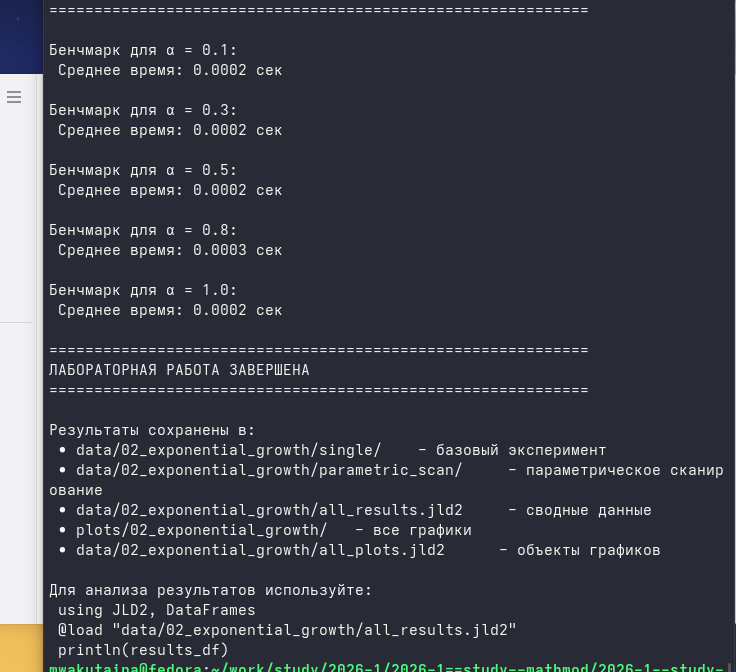
\includegraphics[width=0.7\linewidth,height=\textheight,keepaspectratio]{image/86.png}

}

\caption{\label{fig-070}Выполнение программы}

\end{figure}%

\begin{figure}

\centering{

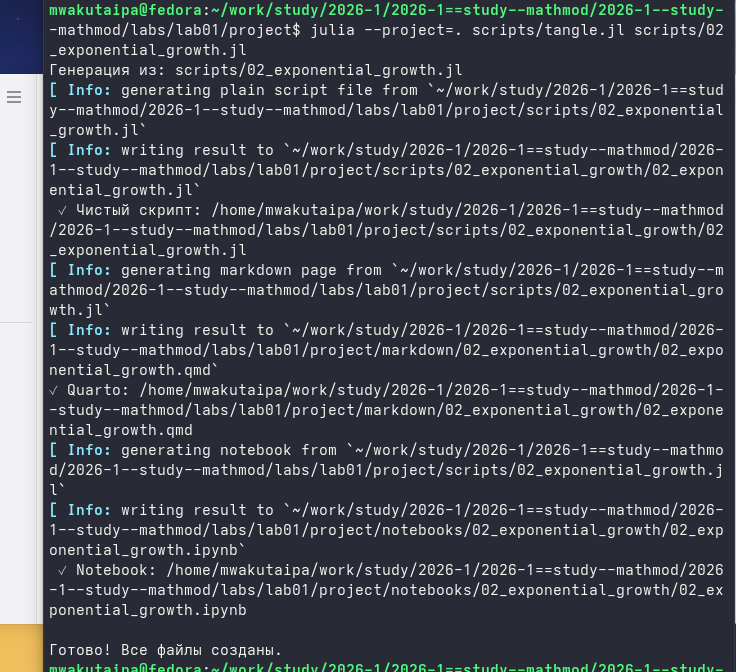
\includegraphics[width=0.7\linewidth,height=\textheight,keepaspectratio]{image/87.png}

}

\caption{\label{fig-071}Создание производные форматы}

\end{figure}%

\chapter{Выводы}\label{ux432ux44bux432ux43eux434ux44b}

При выполнение данной работы я подготовила рабочее пространство и
познакомилась с языком программирования Julia и пакет DrWatson, освоила
основы литературного программирования.

\chapter*{Список
литературы}\label{ux441ux43fux438ux441ux43eux43a-ux43bux438ux442ux435ux440ux430ux442ux443ux440ux44b}
\addcontentsline{toc}{chapter}{Список литературы}

\printbibliography[heading=none]





\end{document}
